\section{Simulation}
\label{sec:simulation}

\par In this section, a brief description of the circuit modeled through NGspice is going to be presented and the values obtained on it are going to be compared with the ones obtained on Octave. The purpose of the simulation was to maximise the merit obtained and, as such, to obtain the values of the gain and central frequency. Furthermore, we'll analise the input and output impedances as well.

\par In order to do that, we started with the circuit previously provided, kept the OP-AMP (as it was supposed to be), and made some changes in the capacitors and resistors, as explained before. Next, both output gain and central frequency were measured, and the respective deviations were computed. The results are shown in the table bellow.

\begin{table}[H]
  \centering
  \begin{tabular}{|l|r|}
    \hline    
   V Gain&34.1403\\ \hline
Bandwidth&1.22339E+06 Hz\\ \hline
Lower Cut Off Freq& 15.8089 Hz\\ \hline
Higher Cut Off Freq& 1.22341E+06 Hz\\ \hline

     \end{tabular}
  \caption{Output gain, central frequency and respective deviations ([dB],[Hz])}
\end{table}
  
\par Following this, we analised the frequency responce of the circuit. In order to do this, we plotted both the gain (in dB) and the phase (in degrees), as functions of the frequency. The plots can be seen in the figures bellow.

\begin{figure}[H]
\centering
\begin{subfigure}{.5\textwidth}
  \centering
  \includegraphics[width=1.1\linewidth]{gain.pdf}
  \caption{Gain as function of frequency}
  \label{fig:sim1}
\end{subfigure}%
\begin{subfigure}{.5\textwidth}
  \centering
  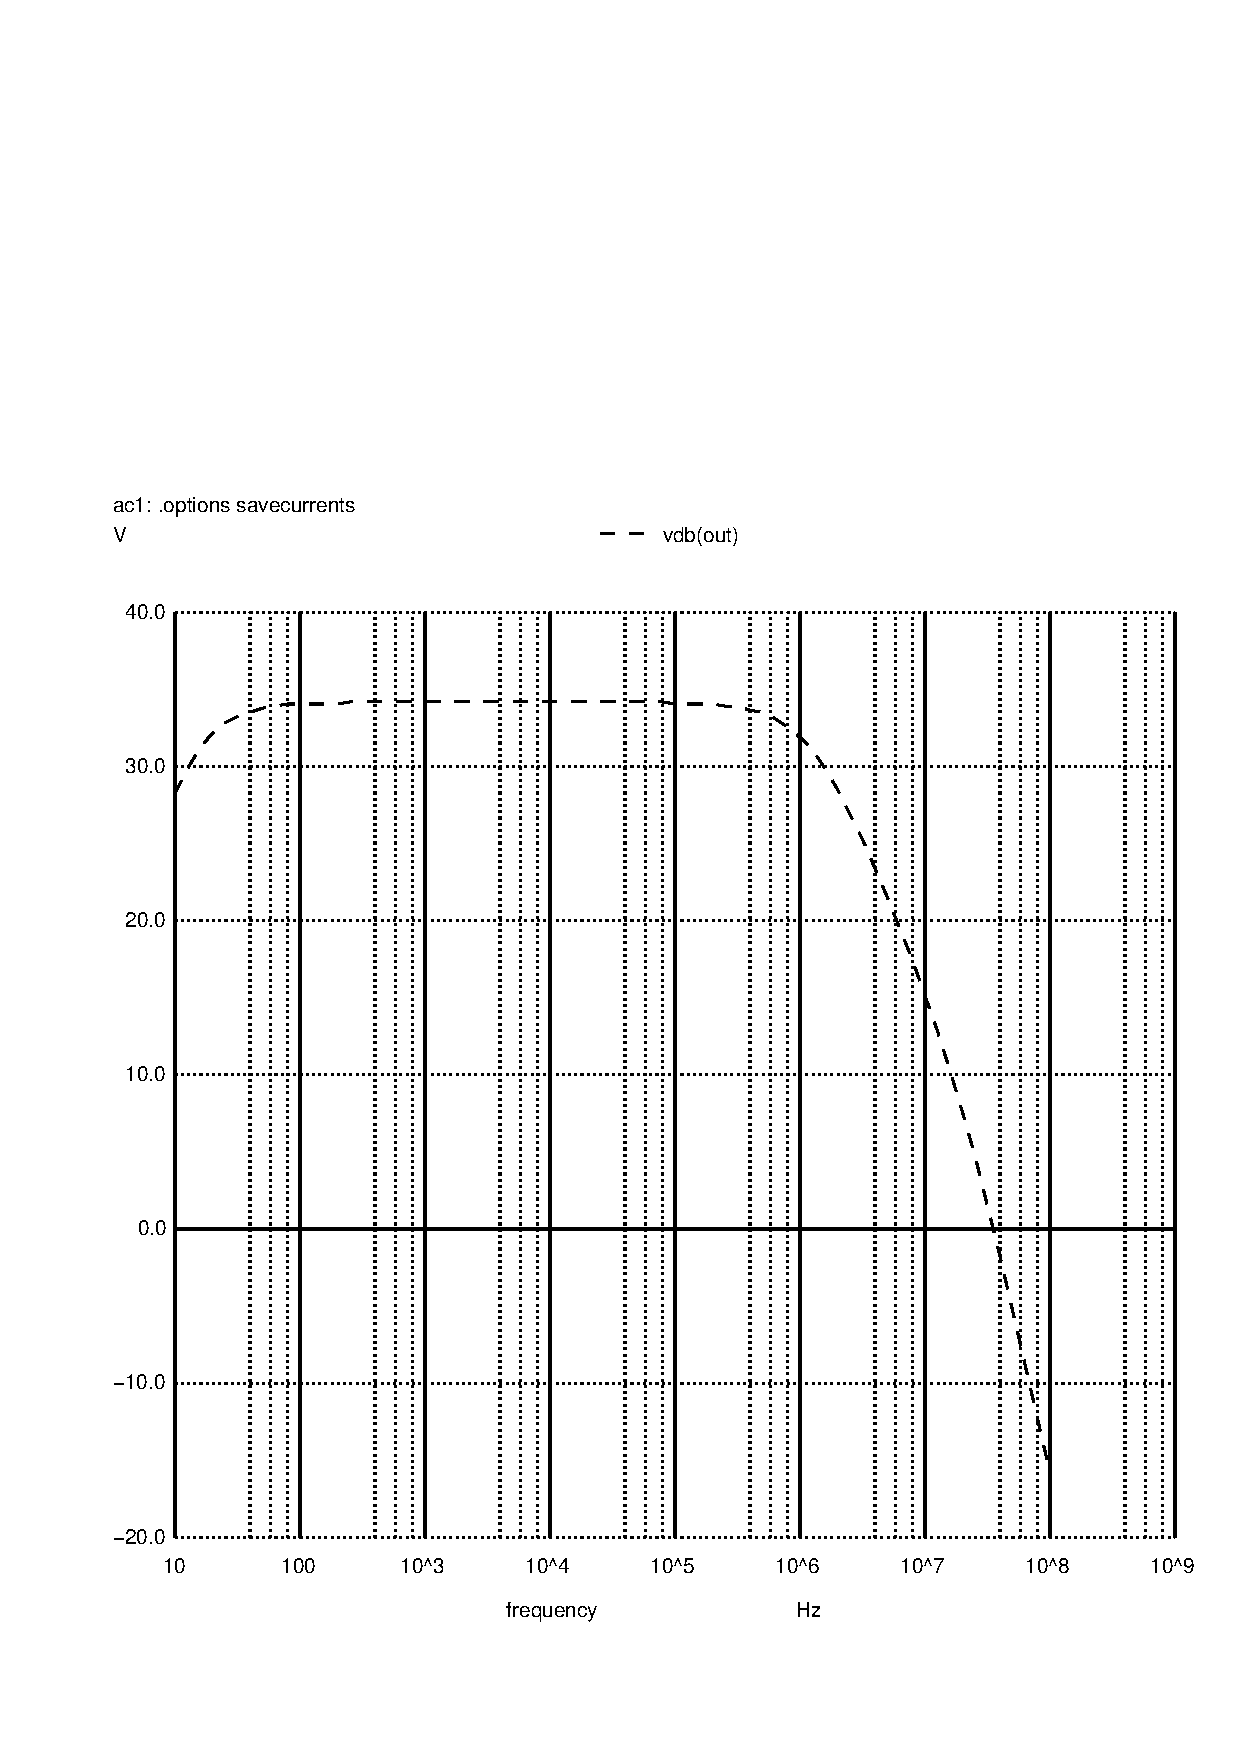
\includegraphics[width=1.1\linewidth]{vo2f.pdf}
  \caption{Phase as funtion of frequency}
  \label{fig:sim2}
\end{subfigure}
\end{figure}

\par The next step was to simulate the input impedance. The obtained value can be seen bellow - as one might confirm, this value is high, which is a requirement to have low voltage degradation at the input.

\begin{table}[H]
  \centering
  \begin{tabular}{|l|r|}
    \hline    
   Zin & -1445.61 + 303.661 j\\ \hline

    \end{tabular}
  \caption{Input impedance of the circuit [$\Omega$]}
    \label{tab:Zin}
\end{table}

\par Besides having a high input impedance, it is also important to have a low output impedance, in order to have low voltage degradation at the output as well. In order to calculate this value, we needed a different setup, which explains the two \textit{.net} files in \textit{sim} folder. The value of the output impedance is shown bellow, and it is very low, as we can see.

\begin{table}[H]
  \centering
  \begin{tabular}{|l|r|}
    \hline    
   \input{../sim/op_ZO_tab}
    \end{tabular}
  \caption{Output impedance of the circuit [$\Omega$]}
    \label{tab:Zout}
\end{table}

\par Finally, in order to evaluate the relation cost/quality of our solution, the figure of merit is presented in the next table.

\begin{table}[H]
  \centering
  \begin{tabular}{|l|r|}
    \hline    
   V Gain&34.1403\\ \hline
Low Cut Off Freq& 15.8089 Hz\\ \hline
High Cut Off Freq& 1.22341E+06 Hz\\ \hline
Bandwidth&1.22339E+06 Hz\\ \hline
Cost & 2198.94 MU\\ \hline
merit & 1201.48\\ \hline

    \end{tabular}
  \caption{Figure of merit}
    \label{tab:Zout}
\end{table}

\newpage
